\documentclass{report}

\usepackage[utf8]{inputenc}
\usepackage[T1]{fontenc}
\usepackage[francais]{babel}
\usepackage{listings}
\usepackage[a4paper]{geometry}
\usepackage{graphicx}
\usepackage[export]{adjustbox}
\usepackage{titlesec}
\usepackage{color}
\usepackage[toc, page]{appendix}
\usepackage{hyperref}

\definecolor{xcodekw}{rgb}{0.75, 0.22, 0.60}
\definecolor{xcodestr}{rgb}{0.89, 0.27, 0.30}
\definecolor{xcodecmt}{rgb}{0.31, 0.73, 0.35}

\titleformat{\chapter}[display]
  {\centering\normalfont\huge\bfseries}
  {\chaptertitlename\ \thechapter}
  {20pt}
  {\Huge}

\geometry{hscale=0.75,vscale=0.85,centering}

\DeclareUnicodeCharacter{00A0}{ }

\lstset{
  frame=tb,
  language=C,
  aboveskip=3mm,
  belowskip=3mm,
  showstringspaces=false,
  columns=flexible,
  basicstyle={\small\ttfamily},
  numbers=none,
  breaklines=true,
  breakatwhitespace=true,
  tabsize=3,
  keywordstyle=\color{xcodekw},
  stringstyle=\color{xcodestr},
  commentstyle=\color{xcodecmt}
}

\renewcommand{\thesection}{\arabic{section}}
\renewcommand\appendixtocname{Annexes}
\renewcommand\appendixname{Annexes}
\renewcommand\appendixpagename{Annexes}

\title{Projet OS}
\author{Youri \bsc{Mouton}, Rémy \bsc{Voet} et Samuel \bsc{Monroe}}
\date{Janvier 2015}

\begin{document}

\maketitle

\chapter{Introduction}

	\section{Introduction}

		Le projet qui fait l'objet de ce rapport est un travail de programmation
		en C système sous UNIX, dans le but d'exploiter de manière pratique les connaissances théoriques acquises au cours de Mme. Masson.
		\newline

		Ce travail consiste en l'écriture de trois programmes distincts autour d'une thématique aéronautique, échangeant des informations entre eux via divers moyens, ceci tout en gérant les éventuels conflits et erreurs liés à ces échanges.\newline
		Ces trois programmes sont :\newline
		\begin{description}
			\item[Tour de controle : ]
			Fait office de \textbf{serveur}, joue le rôle majeur en s'occupant de recevoir les demandes des pilotes, en allant chercher les informations météo fournies par le centre météo, et en renvoyant celles-ci en tant que réponses aux demandes des pilotes.\newline

			\item[Pilote : ]
			Fait office de \textbf{client}, envoie une demande d'information ATIS à la tour de contrôle, récupère cette information et replace une demande si cette information n'est pas intègre.\newline

			\item[Le centre météo : ]
			Programme \textbf{tiers} dans l'application, celui-ci se charge de générer automatiquement des informations ATIS différentes tout au long de son fonctionnement.\newline
		\end{description}

	\section{Rappel de l'énoncé}

		Des pilotes qui souhaitent décoller d’un aéroport non contrôlé ont besoin, pour ce faire, de connaître les informations ATIS. Celles-ci sont accessibles via un serveur.
		Chaque pilote va envoyer au serveur une demande ATIS. Le serveur va lors répondre à cette demande en allant chercher les informations nécessaires dans un fichier ATIS.
		Le pilote va recevoir ces informations et il doit alors obligatoirement répondre au serveur en lui envoyant soit :\newline
		\begin{itemize}
			\item Un ACK OK qui signifie \og informations bien reçues \fg et provoque la fin de la communication
			\item Un NAK KO qui signifie \og informations mal comprises \fg et nécessite de renvoyer les informations.
		\end{itemize}

		Le serveur doit pouvoir gérer un nombre indéfini de pilotes (restons réalistes).
		Le fichier ATIS contenant les informations nécessaires aux pilotes doit être régulièrement mis à jour par le gestionnaire météo.

\chapter{Analyse}

	\section{Plan global de l'application}
		Voici un schéma donnant un aperçu rapide des fichiers constituant l'application, et les interactions entre eux via des liens légendés : \newline

		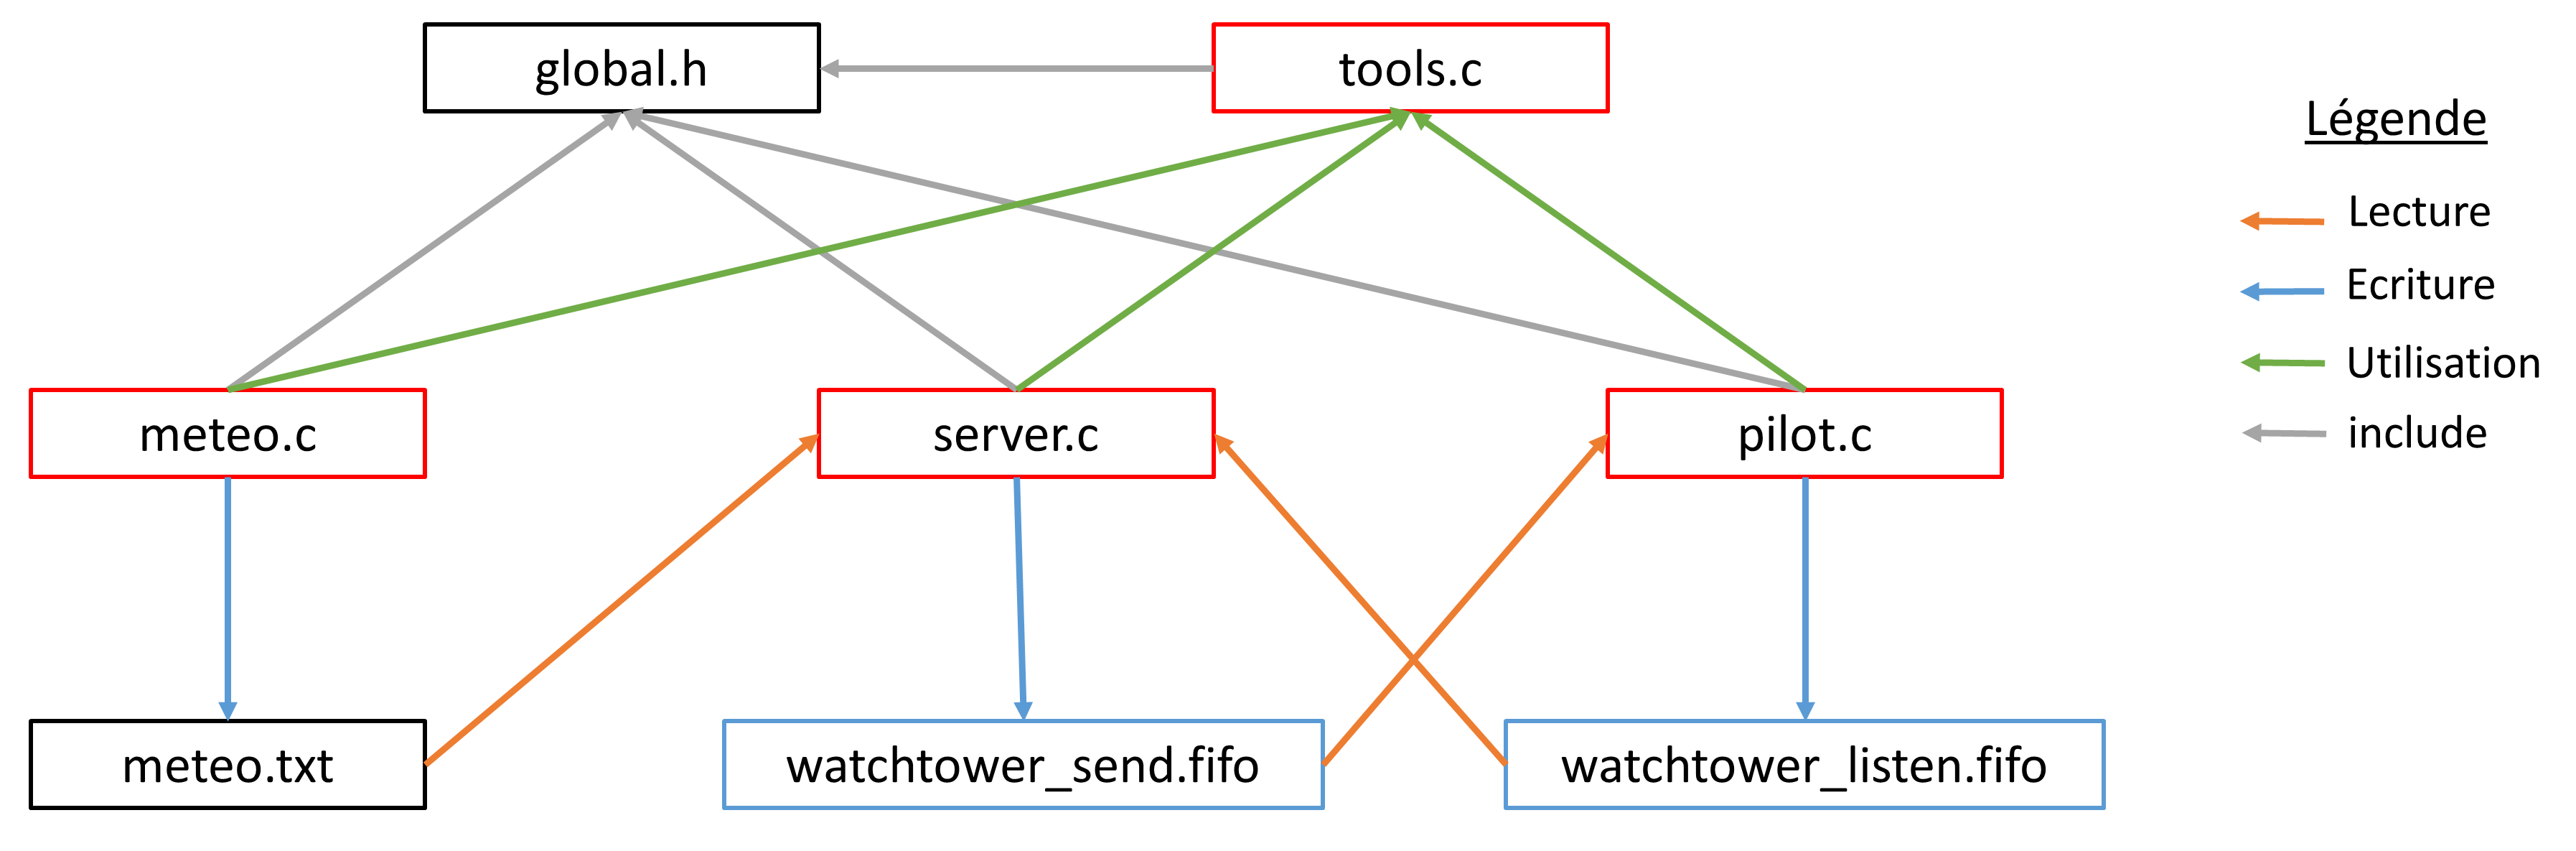
\includegraphics[width=\linewidth, frame]{schemasProjet.png} \newline

		Nos trois programmes qui constituent le coeur de l'application se trouvent sur la ligne au {\textbf{milieu} du schéma, écrits dans les fichiers {\textbf{\color{red} server.c}}, {      \textbf{\color{red} pilot.c}} et {\textbf{\color{red} meteo.c}}.

		Ces programmes vont se servir d' \og outils \fg fonctionnalisés dans le fichier {\textbf{\color{red} tools.c}} et obtenir les librairies, déclarations des fonctions outils et constantes  via inclusion du fichier {\textbf{\color{black} global.h}}.

	\section{meteo.c}

		Lors de la mise en route de l'application, nous commençons par lancer le serveur Meteo.
		Celui-ci possède en son sein un certain nombre d'informations ATIS différentes à utiliser.
		Le serveur Meteo fonctionne sur une succession de boucles, dans lesquelles il va :

		- Sélectionner aléatoirement une des informations ATIS qu'il possède en mémoire.

		- Créer un fichier de verrouillage nommé "lock", afin de spécifier à son environnement qu'il est en train d'opérer.

		- Le serveur ouvre ensuite le fichier "meteo.txt" qui va contenir l'information ATIS actuelle destinée aux autres programmes, si ce fichier n'existait pas, Meteo le crée.

		- Si l'ouverture est un succès, Meteo écrit l'ATIS généré précédemment sur le fichier, ceci en troncature de manière à élimier une autre information ATIS qui est le résultat d'une opération précédente. Cette écriture va durer une seconde, seconde définie par nos soins.

		- Si l'écriture s'est bien déroulée, Meteo supprime le fichier de verrouillage "lock" pour spécifier à l'environnement que l'écriture est terminée et que "meteo.txt" est accessible, et termine la boucle après un repos défini de deux secondes.

	\section{server.c}

		Après l'ouverture du serveur Meteo, nous lançons la tour de contrôle(server.c) ,c'est-à-dire le serveur qui prendra en charge les demandes des pilotes.
		Ce serveur fait divers opérations au lancement, il va notamment : 

		- Créer les deux fichiers fifo : watchtower_send.fifo (fifo Output) et watchtower_listen.fifo (fifo Input).
		Ces deux fichiers sont en fait des points d'entrée et de sortie pour le serveur, l'entrée Input sera celle sur laquelle les pilotes viendront placer leurs requêtes.
		Tandis que la sortie Output sera celle destinée aux envois des réponses à destination des pilotes.

		- Après création, le serveur va ouvrir ces fichiers.

		- Si la création et l'ouverture des fifo est un succès, le serveur peut lancer les opérations. C'est-à-dire prendre en charge les différents pilotes grâce à une boucle de fonctionnement qui va constituer le point principal de la vie du serveur.
		Chaque seconde le serveur lit le fichier fifo Input où les pilotes écrivent leur demande.

		- Les messages pilotes sont traités selon trois cas : requête, confirmation d'acquisition, message invalide.

		- Dans le cas d'une requête ATIS, le serveur lit le fichier meteo.txt qui contient l'ATIS correspondant. Il écrit ensuite cet ATIS sur le fichier fifo Output à l'attention du pilote. 
		Si le fichier meteo.txt est occupé par le serveur Meteo ou qu'il n'existe pas, le serveur renverra un message d'erreur correspondant au pilote qui pourra ensuite reformuler sa demande.

		- Dans le cas d'une confirmation d'acquisiton, le serveur affiche un message signalant qu'un pilote a bien réceptionné sa donnée ATIS, et continue son écoute.

		- Dernier cas, le message est invalide, provoquant une erreur.
 

	\section{pilot.c}
		
		Quand le serveur Meteo et le serveur de la tour de contrôle sont lancés, nous exécutons un certain nombre de pilote qui feront leur demande ATIS à la tour de contrôle.
		Chaque pilote va : 
		
		- Vérifier si le serveur et l'écriture du fifo Input est accessible.
		
		- Après la vérification, écrire sa demande ATIS sur le fifo Input à l'attention de la tour de contrôle.
		
		- Attendre ensuite la réponse du serveur en lisant le fichier fifo Output chaque seconde. Si la réponse est correcte, le pilote envoie un message (ACK) au serveur de confirmation de réception et ensuite "s'auto-detruit".  Si la réponse du serveur n'est pas correcte, le pilote envoie un message (NAK) pour demander au serveur de renvoyer l'ATIS et continue d'attendre la réponse.
		
\chapter{Détails et élements techniques spécifiques}

	\section{Spécificités techniques de l'application}

	\section{Makefile et fichiers de configurations}

	\section{Organisation du travail}

		Nous avons pris le parti d'appuyer, et ce dès les premières lignes de code, notre projet sur le système de versionning "Git" associé
		à un repository en ligne sur le site "Github".
		Cette méthode de travail nous a permis de développer en toute circonstance, en restant à tout moment conscient des nouveaux éléments 
		implémentés par nos pairs et de les prendre immédiatement en considèration.
		Le projet a été lançé aux alentours du 13 Novembre 2014, dans la foulée de l'obtention des consignes de ce travail par Madame Masson.

		Le projet entier, de ses balbutiements à son aboutissement, est disponible à cette adresse : \url{https://github.com/yrmt/OS}

		Concernant le rapport que vous tenez actuellement entre vos mains, nous avons opté pour une rédaction en Latex.
		Nous étions tous trois peu initiés à ce "langage", mais prendre ce parti nous a également permis d'intègrer le rapport
		dans le versionning et ainsi le soumettre aux modifications et améliorations rapides connues sur le projet en lui-même, mais de plus
		ceci nous a permis de prendre de l'expérience avec Latex, atout non-négligeable.

\chapter{Conclusion}
	
	\section{Difficultés rencontrées}

	\section{Solutions apportées aux problèmes}

	\section{Pistes d'améliorations}

	\section{Pour terminer}

\begin{appendices}

\chapter{Code Source}

	\section{global.h}
		\lstinputlisting[language=C]{../global.h}
		\clearpage

	\section{meteo.c}
		\lstinputlisting[language=C]{../meteo.c}
		\clearpage

	\section{server.c}
		\lstinputlisting[language=C]{../server.c}
		\clearpage

	\section{pilot.c}
		\lstinputlisting[language=C]{../pilot.c}
		\clearpage
		
	\section{tools.c}
	 	\lstinputlisting[language=C]{../tools.c}
	 	\clearpage

\end{appendices}

\tableofcontents

\end{document}